\documentclass[tikz,border=16pt]{standalone}
\usepackage{tikz}
\usetikzlibrary{arrows.meta, calc}

\tikzset{
  blk/.style={
    rectangle, draw=black, line width=1.4pt,
    minimum width=3.2cm, minimum height=1.1cm,
    align=center, fill=white,
    font=\small\bfseries\sffamily
  },
  arr/.style  = {-Stealth, line width=1.2pt},
  barr/.style = {Stealth-Stealth, line width=1.2pt},
  darr/.style = {-Stealth, line width=1.0pt, dashed, blue!70},
  lbl/.style  = {font=\scriptsize\sffamily, fill=white, inner sep=1.5pt, align=center},
}

\begin{document}
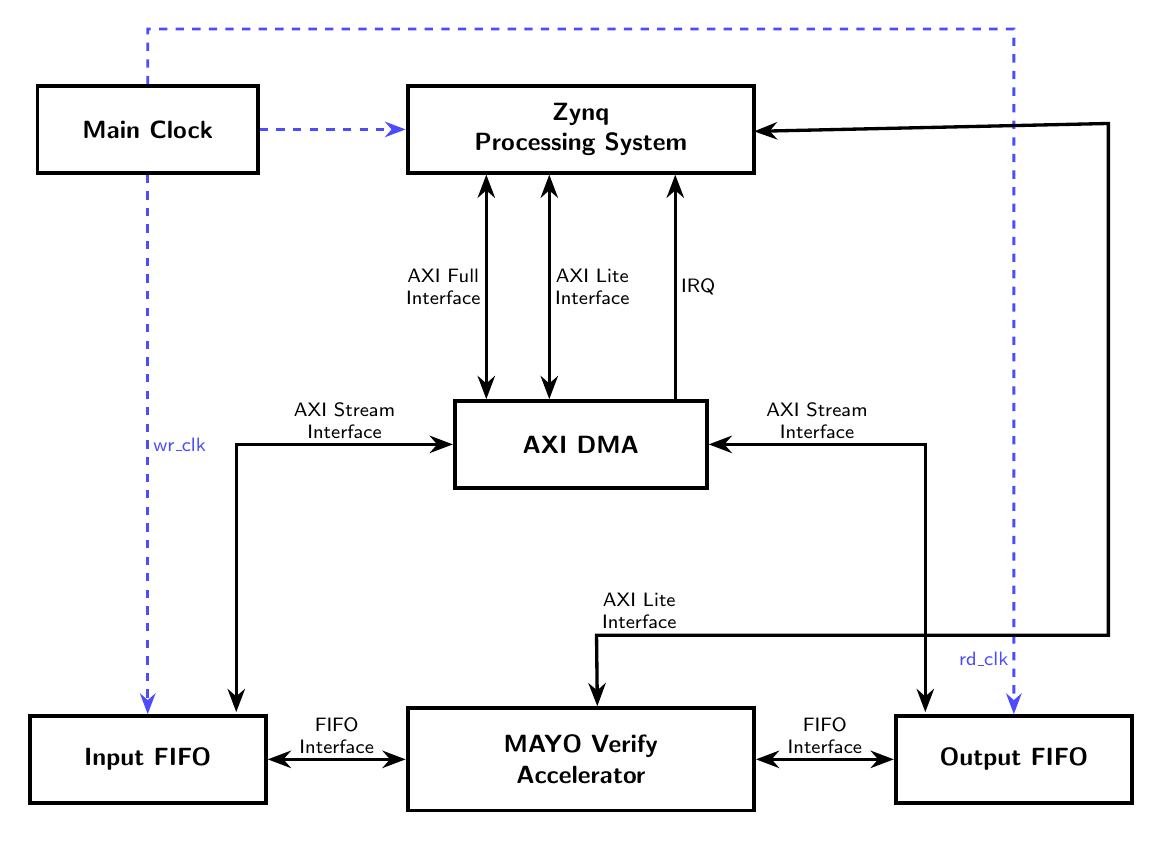
\begin{tikzpicture}

%% ── Row 1: Main Clock (left)  |  Zynq PS (center-right) ─────────────────────
\node[blk, minimum width=2.8cm] (CLK) at (-4.5,  0.0) {Main Clock};
\node[blk, minimum width=4.4cm] (PS)  at ( 1.0,  0.0) {Zynq\\Processing System};

%% ── Row 2: AXI DMA (center) ──────────────────────────────────────────────────
\node[blk, minimum width=3.2cm] (DMA) at ( 1.0, -4.0) {AXI DMA};

%% ── Row 3: Input FIFO | MAYO Verify Accelerator | Output FIFO ───────────────
\node[blk, minimum width=3.0cm] (IFIFO) at (-4.5, -8.0) {Input FIFO};
\node[blk, minimum width=4.4cm, minimum height=1.3cm] (ACC) at (1.0, -8.0) {MAYO Verify\\Accelerator};
\node[blk, minimum width=3.0cm] (OFIFO) at ( 6.5, -8.0) {Output FIFO};

%% ── Main Clock → PS (dashed) ─────────────────────────────────────────────────
\draw[darr] (CLK.east) -- node[lbl, above]{} (PS.west);

%% ── Main Clock → Input FIFO wr_clk (dashed, straight down) ──────────────────
\draw[darr] (CLK.south) -- node[lbl, right]{\textcolor{blue!70}{\scriptsize wr\_clk}} (IFIFO.north);

%% ── Main Clock → Output FIFO rd_clk (dashed, up → across → down) ────────────
\draw[darr] (CLK.north) -- ++(0, 0.7)
    -- ++(11.0, 0)
    -- ++(0, -8.0)
    node[lbl, left]{\textcolor{blue!70}{\scriptsize rd\_clk}}
    -- (OFIFO.north);

%% ── PS ↔ DMA : AXI Full Interface ───────────────────────────────────────────
\draw[barr] ([xshift=-12mm]PS.south)
    -- node[lbl, left]{AXI Full\\Interface}
    ([xshift=-12mm]DMA.north);

%% ── PS ↔ DMA : AXI Lite Interface ───────────────────────────────────────────
\draw[barr] ([xshift=-4mm]PS.south)
    -- node[lbl, right]{AXI Lite\\Interface}
    ([xshift=-4mm]DMA.north);

%% ── DMA → PS : IRQ ───────────────────────────────────────────────────────────
\draw[arr] ([xshift=12mm]DMA.north)
    -- node[lbl, right]{IRQ}
    ([xshift=12mm]PS.south);

%% ── DMA ↔ Input FIFO : AXI Stream (DMA west → left → down to IFIFO north) ───
\draw[barr] ([yshift=0mm]DMA.west)
    -- node[lbl, above]{AXI Stream\\Interface}
    ([xshift=-4mm]IFIFO.east |- DMA.west)
    -- ([xshift=-4mm, yshift=6mm]IFIFO.east);

%% ── DMA ↔ Output FIFO : AXI Stream (DMA east → right → down to OFIFO north) ─
\draw[barr] ([yshift=0mm]DMA.east)
    -- node[lbl, above]{AXI Stream\\Interface}
    ([xshift=4mm]OFIFO.west |- DMA.east)
    -- ([xshift=4mm, yshift=6mm]OFIFO.west);

%% ── Input FIFO ↔ Accelerator : FIFO Interface (horizontal) ──────────────────
\draw[barr] (IFIFO.east)
    -- node[lbl, above]{FIFO\\Interface}
    (ACC.west);

%% ── Output FIFO ↔ Accelerator : FIFO Interface (horizontal) ─────────────────
\draw[barr] (OFIFO.west)
    -- node[lbl, above]{FIFO\\Interface}
    (ACC.east);

%% ── PS ↔ ACC : AXI Lite Control/Status (right spine) ────────────────────────
\draw[barr] ([xshift=22mm, yshift=5.5mm]PS.south)
    % -- ++(0, -0.5)
    -- ++(4.5, 0.1)
    -- ++(0, -6.5)
    -- ++(-6.5, 0)
    -- ([xshift=2.1mm]ACC.north |- ACC.north)
    node[lbl, right, pos=-0.35]{AXI Lite\\Interface};
    -- ([xshift=30mm]ACC.north)

\end{tikzpicture}
\end{document}
